\documentclass[14pt]{extarticle} 
\usepackage{amsmath,mathtools,amsfonts,amsthm,amssymb,hyperref}
\usepackage{wasysym,geometry,bussproofs,latexsym,parskip,bookmark}
\usepackage{mathtools,float}
\newtheorem{defn}{Definition}
\newtheorem{thm}{Theorem}
\newtheorem{claim}{Claim}
\newtheorem{lemma}{Lemma}
\newcommand{\dps}{\displaystyle}
\hypersetup{colorlinks,allcolors=blue,linktoc=all}
\geometry{a4paper} 
\geometry{margin=0.5in}
\title{Math for CS 2015/2019 solutions to ``In-Class Problems Week 14, Wed. (Session 35)''}
\author{https://github.com/spamegg1}
\begin{document}
\maketitle
\tableofcontents

\section{Problem 1}
\subsection{(a)}
\begin{figure}[ht!]
\centering
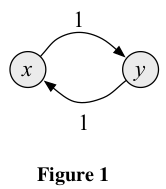
\includegraphics[scale=0.6]{random-walk-1.png}
\end{figure}
Find a stationary distribution for the random walk graph in Figure 1.

\begin{proof}
$d(x) = d(y) = 1/2$
\end{proof}

\subsection{(b)}
Explain why a long random walk starting at node $x$ in Figure 1 will not converge to a stationary distribution. Characterize which starting distributions will converge to the stationary one.

\begin{proof}
It won't converge to a stationary distribution, because you just alternate between nodes $x$ and $y$.
\end{proof}

\subsection{(c)}
\begin{figure}[ht!]
\centering
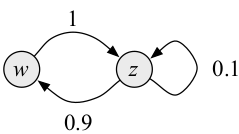
\includegraphics[scale=0.6]{random-walk-2.png}
\end{figure}

Find a stationary distribution for the random walk graph in this figure.

\begin{proof}
$d(w) = 9/19, d(z) = 10/19$. 

You can derive this by setting 

$d(w) = (9/10)d(z)$, 

$d(z) = d(w) + (1/10)d(z)$, and 

$d(w) + d(z) = 1$. 

There is a unique solution.
\end{proof}

\subsection{(d)}
If you start at node $w$ above and take a (long) random walk, does the distribution over nodes ever get close to the stationary distribution? You needn’t prove anything here, just write out a few steps and see what’s happening.

\begin{proof}
Yes, it does.
\end{proof}

\subsection{(e)}
\begin{figure}[ht!]
\centering
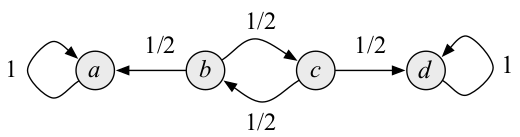
\includegraphics[scale=0.6]{random-walk-3.png}
\end{figure}
Explain why the random walk graph in this figure has an uncountable number of stationary distributions.

\begin{proof}
For any real number $0 < p < 1$ there is a stationary distribution: $d(b) = d(c) = 0$, $d(a) = p$, $d(d) = 1-p$.
\end{proof}

\subsection{(f)}
If you start at node $b$ in the last figure and take a long random walk, the probability you are at node $d$ will be close to what fraction? Explain.

\begin{proof}
1/3.
\end{proof}

\subsection{(g)}
Give an example of a random walk graph that is not strongly connected but has a unique stationary distribution. Hint: There is a trivial example.

\begin{proof}
\begin{figure}[ht!]
\centering
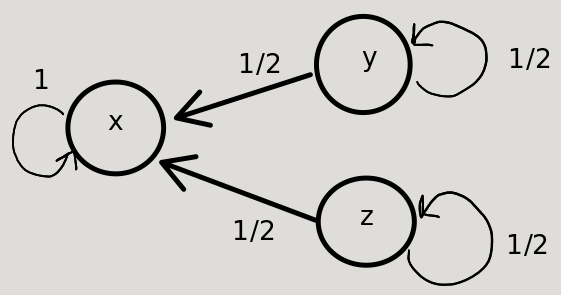
\includegraphics[scale=0.4]{stationary.png}
\end{figure}
Consider this graph. It's not strongly connected (there is no directed path between $y$ and $z$).

To solve for the stationary distribution, we have the equations:
$$
\begin{array}{ccc}
x&=&x \cdot 1\\
y&=&(1/2)\cdot y\\
z&=&(1/2)\cdot z\\
\end{array}
$$
The last two equations force $y = z = 0$, which forces $x = 1$. This is a unique solution, so it's a unique stationary distribution.
\end{proof}

\section{Problem 2}
Prove that for finite random walk graphs, the uniform distribution is stationary iff the probabilities of the edges coming into each vertex always sum to 1, namely
$$
\sum_{u \in \text{into}(v)} p(u,v) = 1
$$
where into$(w) \Coloneqq \{v\,\, | \,\,\langle v \to w\rangle \text{ is an edge}\}$.

\begin{proof}
1. Assume $G$ is a finite random walk graph with vertex set $V = \{v_1, \ldots, v_n\}$.

2. Assume the uniform distribution Pr[at $v_i] = \frac{1}{n}$ on $G$ is stationary. 

Want to prove $\dps\sum_{u \in \text{into}(v_i)} p(u,v_i) = 1$ for all $1 \leq i \leq n$.

3. Since the distribution is stationary, Pr[at $v_i$] = Pr[go to $v_i$ at next step]. 

So by (2) we have $\frac{1}{n}$ = Pr[go to $v_i$ at next step].

4. Notice that by definition, Pr[go to $v_i$ at next step] = $\dps\sum_{u \in \text{into}(v_i)} (p(u,v_i) \cdot Pr[\text{at } u])$. 

So we have $\dps\frac{1}{n} = \sum_{u \in \text{into}(v_i)} (p(u,v_i) \cdot Pr[\text{at } u])$ by (3).

5. Again, since the distribution is stationary, Pr[at $u$] = $\frac{1}{n}$ for all $u \in \text{into}(v_i)$ and all $1 \leq i \leq n$.

6. Combining 4,5 we get $\dps\frac{1}{n} = \sum_{u \in \text{into}(v_i)} (p(u,v_i) \cdot Pr[\text{at } u]) = \frac{1}{n} \cdot\sum_{u \in \text{into}(v_i)} p(u,v_i)$.

7. Cancelling $1/n$ we get $\dps\sum_{u \in \text{into}(v_i)} p(u,v_i) = 1$.

8. Conversely, assume $\dps\sum_{u \in \text{into}(v_i)} p(u,v_i) = 1$ for all $1 \leq i \leq n$. 

Want to prove that the uniform distribution Pr[at $v_i] = \frac{1}{n}$ on $G$ is stationary. 

The proof is very similar to the above steps.
\end{proof}

\section{Problem 3}
A Google-graph is a random-walk graph such that every edge leaving any given vertex has the same proba­bility. That is, the probability of each edge $\langle v \to w \rangle$ is 1/outdeg$(v)$.

A digraph is symmetric if, whenever $\langle v \to w\rangle$ is an edge, so is $\langle w \to v\rangle$. Given any finite, symmetric Google-graph, let $d(v) \Coloneqq$ outdeg$(v) / e$ where $e$ is the total number of edges in the graph.

\subsection{(a)}
If $d$ was used for webpage ranking, how could you hack this to give your page a high rank? ...and explain informally why this wouldn’t work for “real” page rank using digraphs?

\begin{proof}
???
\end{proof}

\subsection{(b)}
Show that $d$ is a stationary distribution.

\begin{proof}
1. Assume there are $e$ edges in total in the graph $G$. We need to show for evert vertex $v$: Pr[at $v$] = Pr[go to $v$ at next step]. Assume $v$ is a vertex in $G$.

2. By the definition of our distribution we have Pr[at $x$] = $d(x)$ = outdeg$(x) / e$ for all vertices $x$. In particular Pr[at $v$] = $d(v)$ = outdeg$(v)/e$.

3. Since $G$ is symmetric, outdeg$(x)$ = indeg$(x)$ for all vertices $x$. So in particular,\\ Pr[at $v$] = indeg$(v)/e$.

4. Also remember that by definition of a Google-graph we have $p(u,v) = 1/$outdeg$(u)$ for all other vertices $u$.

5. Then by (2), (3), (4), Pr[go to $v$ at next step] is equal to:
$$
\sum_{u \in \text{into}(v)} Pr[\text{at }u] \cdot p(u,v) = \sum_{u \in \text{into}(v)} \frac{\text{outdeg}(u)}{e} \cdot \frac{1}{\text{outdeg}(u)} = \frac{|\text{into}(v)|}{e} = \frac{\text{indeg}(v)}{e}
$$
6. By (3) and (5) we see that Pr[at $v$] = indeg$(v)/e$ = Pr[go to $v$ at next step]. So $d$ is a stationary distribution.
\end{proof}

\end{document}
